\documentclass[MASTER.tex]{subfiles} 
\begin{document} 

%=======================================================================%
 
  
\textbf{Decision Trees}
 
   Decision Trees (DTs) are a non-parametric supervised learning method used for classification and regression.  The goal is to create a model that predicts the value of a target variable by learning simple decision rules inferred from the data features.
 
 

 
 A decision tree is a simple representation for classifying examples. Decision tree learning is one of the most successful techniques for supervised classification learning[citation needed]. For this section, assume that all of the features have finite discrete domains, and there is a single target feature called the classification. Each element of the domain of the classification is called a class. 
 
%=======================================================================%
 
  
 \textbf{Decision Trees}
  
   A decision tree or a classification tree is a tree in which each internal (non-leaf) node is labeled with an input feature. 
   The arcs coming from a node labeled with a feature are labeled with each of the possible values of the feature.
   Each leaf of the tree is labeled with a class or a probability distribution over the classes.

 
 
%=======================================================================%
 
  
\textbf{Decision Trees}
 
\item For instance, in the example below, decision trees learn from data to approximate a sine curve with a set of \textit{If-Then-Else} decision rules. 
\item The deeper the tree, the more complex the decision rules and the fitter the model.
 

 
%========================================================================= %
 [fragile]
  
\textbf{Decision Trees}\\

Using the Iris dataset, we can construct a tree as follows:
{
\normalsize
\begin{framed}
\begin{verbatim}
>>> from sklearn.datasets import load_iris
>>> from sklearn import tree
>>> iris = load_iris()
>>> clf = tree.DecisionTreeClassifier()
>>> clf = clf.fit(iris.data, iris.target)
\end{verbatim}
\end{framed}
}
 
%========================================================================= %

 

\begin{figure}
\centering
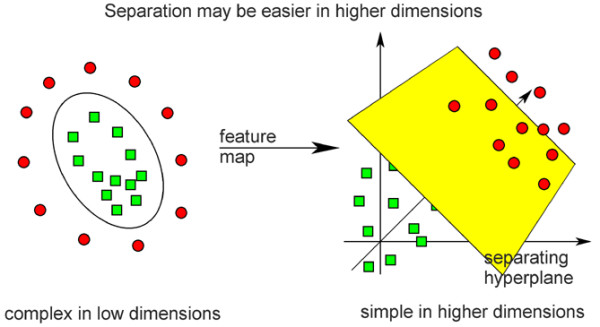
\includegraphics[width=1.1\linewidth]{SVMexplain}
\end{figure}
 
 

\end{document}